\documentclass[conference]{IEEEtran}
\IEEEoverridecommandlockouts
% The preceding line is only needed to identify funding in the first footnote. If that is unneeded, please comment it out.
\usepackage{cite}
\usepackage{amsmath,amssymb,amsfonts}
\usepackage{algorithmic}
\usepackage{graphicx}
\usepackage{textcomp}
\usepackage{float}
\usepackage{url}
\usepackage{listings}

\usepackage{colortbl}
%\usepackage{multirow}
%\usepackage{booktabs}



\definecolor{CEWebSHeading}{cmyk}{0,0,0,0.13}
\definecolor{CEWebSImportant}{cmyk}{0,0,0,0.05}
\definecolor{CEWebSUrgent}{cmyk}{0,1,1,0.13}
\definecolor{CEWebSBad}{cmyk}{0,0.25,0.25,0}
\definecolor{CEWebSGood}{cmyk}{0.25,0,0.25,0}
\definecolor{CEWebSNeutral}{cmyk}{0.25,0.25,0,0}

\definecolor{white}{rgb}{1.0,1.0,1.0}
\definecolor{black}{rgb}{0.0,0.0,0.0}

\definecolor{darkblue}{rgb}{0.0,0.0,0.6}
\definecolor{darkred}{rgb}{0.6,0.0,0.0}
\definecolor{darkgreen}{rgb}{0.0,0.6,0.0}
\definecolor{light-gray}{rgb}{0.95,0.95,0.95}

\lstloadlanguages{ XML, SQL, Java, bash, Ant }
\lstset{
		language=XML,
    backgroundcolor=\color{light-gray},		
    basicstyle=\ttfamily\scriptsize\color{black},
%    commentstyle=\itshape\color{darkgreen}, %tiny, scriptsize
%    keywordstyle=\bfseries\color{darkblue},
%    stringstyle=\color{darkblue},  		
%    frameround=fttt,
%    frame=trBL,
%    float=hbtp,
    frame=single,
    framerule=0.4pt,
		numbers=none,
    columns=fixed,
    numberstyle=\tiny,
		extendedchars=true,
    columns=flexible,
    tabsize=2,
    showspaces=false,
    showstringspaces=false,
    breaklines=true,
    breakautoindent=true,
    captionpos=b
}

\def\BibTeX{{\rm B\kern-.05em{\sc i\kern-.025em b}\kern-.08em
    T\kern-.1667em\lower.7ex\hbox{E}\kern-.125emX}}
\begin{document}

\title{N2Sky - A Neural Network Problem Solving Environment Fostering Virtual Resources}

\author{\IEEEauthorblockN{Andrii Fedorenko}
\IEEEauthorblockA{\textit{University of Vienna} \\
Vienna, Austria \\
andriifedorenko@gmail.com}
\and
\IEEEauthorblockN{Aliaksandr Adamenko}
\IEEEauthorblockA{\textit{University of Vienna} \\
Vienna, Austria \\
alexadamenko@gmail.com}
\and
\IEEEauthorblockN{Erich Schikuta}
\IEEEauthorblockA{\textit{University of Vienna} \\
Vienna, Austria \\
erich.schikuta@univie.ac.at}
}

\maketitle

\begin{IEEEkeywords}
Neural Networks, Problem Solving Environment, Cloudcomputing, Containers, Microservices
\end{IEEEkeywords}

\begin{abstract}

This paper presents the novel N2Sky system, which provides a virtual collaboration platform to the computational intelligence community.
It realizes the Neural Networks as a Service paradigm allowing to share and exchange neural network knowledge resources on a worldwide basis by a transparent environment fostering state-of-art hardware and software infrastructures.
The system is motivated by the goal to deliver an intuitive tool for different stakeholders of the neural network community, as arbitrary users, looking for a packaged neural network solution to a given problem, neural network engineers, creating and training their own neural network object based on available paradigms, and experienced neural network contributors, developing and implementing their own neural network type and sharing it with the community.

To meet these targets N2Sky provides an intuitive user interface which embodies latest web technology to make the user's interaction as simple and efficient as possible.
Fostering cloud resources N2Sky is based on container-based virtualization technology to provide for higher flexibility, portability, dynamic orchestration, and performance.
We give the motivation and design goals for the new system, describe its architectural layout and technical specifics, and present use cases for the different user types.

\end{abstract}

\section{Introduction}
\label{sec:introduction}

A virtual organization/community platform~\cite{FoKeTu01} is a medium for human beings, organizations or enterprises to share different types of geographically distributed information (domain specific knowledge) or computational infrastructure (computing nodes, storage systems, databases, libraries and special purpose scientific instruments).
This enables more effective and seamless collaboration of scattered communities, both commercial and scientific, enabling large-scale applications and transparent access to high-end resources from the desktop.

The driving stimulus for the development of science is the exchange of information and resources between researchers.
As the fields of computational intelligence and machine learning mature, there is a growing need to provide
researchers with the ability to exchange information, share resources, discuss
problems and new directions, and learn about other's work. The limitations of
traditional scientific communication inspired to create virtual communities to gather research, education, and application-oriented resources.
The goal of the community is to create a place
where scientists, students, and the general public can work together despite any of
their geographic limitations. Anyone who is interested can share research, obtain
resources, or simply learn more about computational intelligence.

However, in the domain of neural network research, we see this target only insufficiently met until now.
In our preceding research, we designed and developed N2Sky~\cite{N2Sky}, a virtual platform aiming for the computational intelligence (CI) community, which enables access to neural network knowledge and fosters virtualized computing resources. Though, due to design decisions then, this original system did not allow to follow the ongoing shift in cloud computing easily. Also, the focus on one classical programming paradigm made it difficult to provide the experience of today's user interface technology.

Therefore, in this paper, we present the new N2Sky system, which realizes the \emph{Neural Networks as a Service} paradigm allowing to share and exchange neural network knowledge resources on a worldwide basis by a transparent environment fostering state-of-art hardware and software infrastructures.
Hereby provides N2Sky a neural network solution stack with specific capabilities to its different stakeholders. We focus on three main groups of users with different motivations using N2Sky:

\begin{itemize}
  \item The arbitrary \emph{Neural Network User} is searching for packaged neural network solutions for given problem domains and an execution framework providing computational resources for analysis of the user's provided data representing the problem.
  \item The \emph{Neural Network Engineer} shows profound neural network knowledge and is looking for a comfortable simulation environment for artificial neural networks. Here a development stack is needed which allows creating new neural network objects based on available paradigms and gives access to easy to use powerful computational resources for network training. Further capable data management mechanism has to be available for network and training data storage.
  \item The \emph{Neural Network Contributor} represents the neural network scientist who envisions new neural network paradigms and aims for sharing findings with the community. This goal asks for mechanisms, which allow to code, deploy and analyse the new network paradigm and to describe its semantics by a domain specific standardized language for easy distribution in the community.
\end{itemize}

The structure of the paper, is as follows: In section~\ref{sec:SOTA} the state of the art of neural
network simulation environments and the baseline research is presented. In section~\ref{sec:architecture} we identify the shortcomings of the original N2Sky system, derive our new technical design decisions and present the new micro-service and container-based architecture. The new user interface is introduced in section~\ref{sec:interface}, which follows the responsive design paradigm and fosters latest web technologies.
Use cases for the different user types are presented in section~\ref{sec:usecases}, which give an impression of the user's experience working with the new system.
Finally, the paper concludes our findings and presents our plans for future work.

\section{Related Work and Baseline Research}
\label{sec:SOTA}

The driving stimulus for development in the computational science domain is the exchange of knowledge
and resources between researchers. This principle is just as valid for any other research community too.

The UK e-Science initiative~\cite{UKeS} describes several
goals to be reached by fostering new stimulating techniques:

\begin{itemize}
  \item Enabling more effective and seamless collaboration of dispersed communities, both scientific and commercial.
  \item enable large-scale applications comprising of thousands of computers, large-scale pipelines etc.
  \item Transparent access to “high-end” resources from the desktop.
  \item Provide a uniform “look \& feel” to a wide range of resources
  \item Location independence of computational resources as well as data. 
\end{itemize}

However, these targets are not reached in the computational intelligence community until now.
As an example, we examine the situation of neural network simulation.
Over the last decades, a very large number of artificial neural network simulation environments have been developed, which aim to mimic the behaviour biological neural networks~\cite{prieto2016neural}. It started with systems which were developed for specific network families, as Aspirin/MIGRAINES
\cite{Lei91}, SOM-PAK \cite{som92}. Some systems aimed for a more comprehensive environment, as SNNS~\cite{Zel92}.
New technology shifts enabled new concepts, as distributed cooperative environments over the Internet, as NeuroWeb~\cite{schikuta2002neuroweb}.
With the advance of virtual resources by Grid and Cloud computing new collaborative environments motivated the authors of this paper to aim for an "everything about sharing" approach leading the way towards virtual collaborative organisations, as N2Grid~\cite{schikuta2004n2grid} and N2Cloud~\cite{huqqani2010n2cloud}.

However, all these systems, reaching from programming language extensions over proprietary stand alone systems to distributed platforms, share the
same common problems:

\begin{itemize}

\item  \emph{Complex tool}, which mostly do not present an intuitive interface to the user.
\item  \emph{Proprietary system} with missing interconnection and data exchange to other software systems.
\item  \emph{Lacking} provisioning of arbitrary \emph{computing resources}, as CPUs, disks, network, on demand.
\end{itemize}


These problems lead to the situation that quite a number of simulation systems exist, but which are rarely
used. Hence, scientists invent the wheel over and over again and develop their own neural network systems for their specific
needs. We believe that this situation is one of the reasons for an obstructed open information and data exchange within the scientific community.

A promising project, totally in line with our motivation, was the CIML (Computational Intelligence and Machine Learning) community~\cite{zurada2009building}. The goal of CIML was to create an online virtual scientific community wherein anyone interested in computational intelligence and machine learning can share research, obtain resources, or simply learn more. Sorry to say, but CIML failed. One reason was that CIML targeted a too huge and dispersed community and offered too many and different resources. Due to lack of automated guidance of the System, it was difficult for the user "to find its specific needle in the haystack".

Having this situation in mind we realized N2Sky~\cite{N2Sky}, with a clear focus on neural networks aiming for intuitive user guidance and transparent resource access.
N2Sky was designed as an artificial neural network provisioning environment facilitating the users to create, train, evaluate neural networks fostering different types of computing resources. The system is Cloud based in order to allow for a growing virtual user community.
N2Sky supports experienced users to easily run their simulations by accessing data related neural network objects. Moreover, N2Sky provides a facility to end users to solve their problems by using predefined objects and paradigms. For the purpose of thin clients a simple Web browser, which can execute on a PC or a smart phone, can be used to access the front-end, the N2Sky (Mobile) Web Portal. %It is relying on the N2Sky user management service which grants access to the system. %Figure~\ref{fig:N2Sky} shows, the N2Sky login screen on an iPhone and a Mac as example for this portability issue~\cite{N2Sky}.
N2Sky aroused strong interest even beyond the computational intelligence community\footnote{http://cacm.acm.org/news/171642-neural-nets-now-available-in-the-Cloud/}.

The pillar of our envisioned system is ViNNSL, the Vienna Neural Network Specification Language~\cite{Beran2008}. It is key for easy sharing of resources between the paradigm provider and the customers. ViNNSL is an XML-based domain specific language providing mechanisms to specify neural network objects in a standardized way by attributing them with semantic information. Originally it was developed as communication framework to support service-oriented architecture based neural network environments. Even more, ViNNSL is capable of describing the static structure, the training and execution phase of neural network objects in a distributed infrastructure, as grids and clouds.
Its last extension~\cite{ijcnn15} supports semantic information too, describing the usage scenario of network objects for given problem domain.

The following short example illustrates the use of ViNNSL. The listing~\ref{vinnsl_definition} defines 
a 2-5-1 backpropagation network for the well-known XOR problem. Besides the description of the structure of the network, also the application domain for using this network is specified. This is the basis for smart searching of feasible neural networks for given problems.

\lstset{language=XML}
\begin{lstlisting}[float,caption={ViNNSL: XOR-Backpropagation Neural Network Definition},label={vinnsl_definition}]
<definition xmlns="http://www.pri.univie.ac.at/../vinnsl">
  <identifier>7</identifier>
  <problemdomain>
    <backpropagation/>
    <classifier/>
      <XOR-net/>
    </classifier>
  </problemdomain>
  <executionenvironment>
  ...
  </executionenvironment>
  <structure>
    <input>
      <id>Input1</id>
      <dimension>2</dimension>
      <size>1</size>
    </input>
    <hidden>
      <id>Hidden1</id>
      <dimension>5</dimension>
      <size>1</size>
    </hidden>
    <output>
      <id>Output1</id>
      <dimension>1</dimension>
      <size>1</size>
    </output>
    <connections>
      ...
    </connections>
  </structure>
  <parameters>
    <valueparameter>
      <name>lrate</name>
      <label>Learning Rate</label>
      <value>0.3</value>
    </valueparameter>
    ...
  </parameters>
</definition>\end{lstlisting}


\section{A Micro-Kernel Container-based System Architecture}
\label{sec:architecture}

Service migration to the cloud in the recent years is a clear trend in the IT-industry, and it is not surprising that some of the companies are trying to leverage existing cloud infrastructure to bring deep and machine learning solutions to the market. IBM SPSS, Amazon AWS, Google Cloud AI services are meant to provide software tools to the different stakeholders, but they are primarily focusing on the business users, which primary goal is to use applied statistics techniques to fulfill existing business needs. Services are split into components, each of which hides internal implementation of the solution and provides an interface for a specific task: speech recognition, text analysis, etc. Variety of pricing models, a necessity to use other software products of the company, proprietary code and low level of scalability and extensibility are making these products less attractive for the scientific and academic community. Vendor lock-in and inability to control execution and development process are making such software systems and services non-flexible and nontransparent, leading to the scenario where each service provider tends to aggregate and try to sell as many proprietary services as possible.

We consider these aspects as limiting factors for the development of the framework. We believe that such properties as an ability to share knowledge and resources, re-usage of the existing solutions and collaborative work are key features which should be put as a foundation of distributed neural network execution platform.

Keeping that in mind, we tried to re-design the existing solution N2Sky, where new architecture and usability solutions are reflecting core functional ideas of cloud-based execution environments.

N2Sky was designed to provide natural support for cloud deployment with distributed computational resources. However, N2Sky was intended as a single monolithic application written in Java, which is not well aligned with cloud infrastructure and virtual organization concepts -- high redeployment costs, low level of extensibility, the necessity to understand the application code to experiment with neural networks objects and poor computational distribution capacities.

That is why we have decided to put microservices ~\cite{micro} approach as a foundation of the new architectural design. The main idea of the microservices approach is to decompose the software system functionality into separate components, which are responsible for specific tasks. Each component runs in its own isolated environment which is achieved by using Linux containers (LXC)~\cite{LXC} and Docker~\cite{docker}. All the components are interacting with each other through the API, so they are not aware of any internal implementation details. It allows to have a scalable architecture, which can be easily extended or modified by introducing new modules or changing the existing ones -- the only thing developer should care about is proper communication between components.

As the previous system was developed as a Java application, it was entirely language dependent -- to apply any changes to the neural network execution engine or introduce new neural network object or paradigm, and a developer was restricted to Java language. The new design allows developers and researchers to introduce both system modules and neural networks implementations in any language of their choice: the only restriction is to provide API to communicate with. Making small adjustments to the existing Docker image, adding train and test endpoints and the neural network is deployed and ready to be used.

Microservice architecture brings additional advantage -- load balancing, which comes from the symbiosis of shared cloud resources and microservices. In case, if there is a computational demand, the scalability is achieved by merely running new container -- secure and robust solution, which was not possible in the monolithic approach as spawning a new instance with a whole application is a noticeable overhead.

Container quantity can grow very fast; it becomes clear that manual maintenance of dozens, or even millions of Docker containers can be a tough task, especially considering a cloud environment. For that reason, we’ve decided to use container orchestration software as Cloudify~\cite{cloudify}. This tool is providing high-level interfaces to communicate with cloud-based platforms and control deployment and execution of containers.

Putting all these technologies and design approaches together, we receive a robust and efficient cloud-based environment, which can be easily scaled both horizontally and vertically.

The current working version of the new architecture is presented in figure~\ref{fig:arch}.

\begin{figure}[H]
  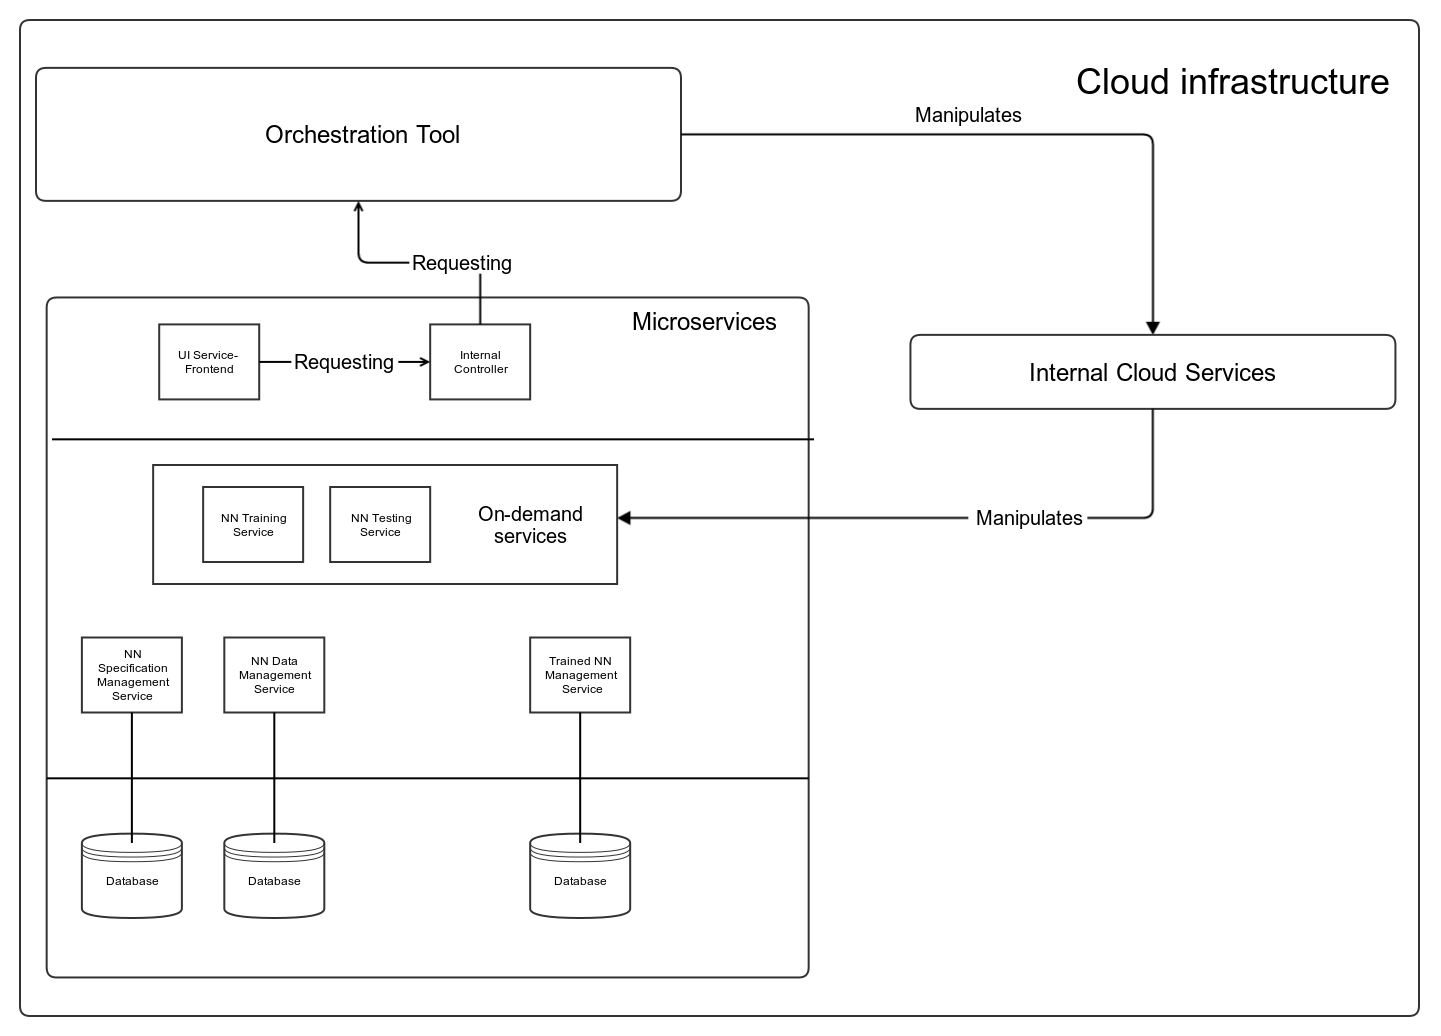
\includegraphics[width=\linewidth]{architecture.png}
  \caption{New N2Sky architechture}
  \label{fig:arch}
\end{figure}

Communication between components of the system is performed as follows:
\begin{itemize}
\item Internal controller is responsible for handling user requests, controlling them and either submitting them to the orchestration tool to spawn new container or using the existing instance of the requested resource,
\item Orchestration tool is responsible for interacting with cloud infrastructure and spawning new instances of neural network objects and internal services,
\item On-demand services is pool of neural network objects instances, which can be used for training and testing using the provided data,
\item Neural network data archive is a separate service on top of the database. It will provide a specific API to add any external data source,
\item Neural specification management service is a component which is responsible for managing existing neural network paradigms, used for instantiation of neural network objects, and
\item Trained NN Management Service is responsible for saving and retrieving trained neural network object, in case a user wants to use pre-trained neural networks.
\end{itemize}

\section{Novel User Centered Interface}
\label{sec:interface}

The user-centered design is a fundamental requirement for N2Sky. Looking back on past experiences with the application, there were identified the real capabilities and needs of users. N2Sky was moved from a complex expert system to an easily understandable application. Every interested user without having deep knowledge in the neural network field can freely use N2Sky.  The goal was to save and gain the current functionality of the application and decrease the visual complexity of it.

\subsection{Frontend and services}

N2Sky today is a cross-platform handy application with responsive design. The frontend is written on the ReactJS framework and it is convertible to the React-Native framework. The application is accessible from desktop computers, as well as from mobile devices or other devices with any operational system. Furthermore, the backend has the microservices architecture to support scalability. Each of the microservices is developed on NodeJS server, which implies efficiency and lightweight. This architecture enables its users to freely and easily work with the application without interruptions or waiting until it is completely loaded.

\subsection{Modular design}
The central concept of the application is to support the Software as a Service (SaaS) and Platform as a Service (PaaS) distributions.  N2Sky consists of two modules: administration module and main application module.

\paragraph{Administration module} The administration module allows the system administrator to control the environment. The module supports OpenStack and Cloudify monitoring. Managing is possible through the application dashboard. It also contains custom monitoring and an alerting management system, which can be installed on any server within the N2Sky user interface. The administration module implements PaaS. It is fully configurable and wrapped into the open source project to make the module accessible to third-party applications.
\paragraph{Main application module} The main application module is the central neural network user module of N2Sky. Within this module, users can use, train and test existing neural networks. It is possible to reuse the neural network paradigms and create own neural network. N2Sky allows deploying own networks and store data in the cloud. Module services are supporting the SaaS distribution. Experts can use an application directly through the N2Sky API, or they can integrate N2Sky services into their own application.

\subsection{User roles}

In order to make the N2Sky user interface intuitive for arbitrary users as well as advanced professional users, it was decided to separate the user roles. Every user role has its own way of interaction with the application:
\begin{itemize}
\item \emph{The arbitrary neural network user.} Such a user has no necessity to have deep knowledge of the neural network field or know any programming language. The main goal of the arbitrary user is to find neural network solvers to given problems and to study found neural networks within N2Sky. The contributor has access only to his own dashboard and public available resources on the main application module. He can perform semantic search for available neural network paradigms and use them.
\item \emph{The neural network engineer.} He has the same options as the arbitrary user but he can also create and train new running neural network instances and test them. This user can share his trained neural network by making it public.
\item \emph{The neural network contributor} is an expert user, which has enough knowledge and experience to create his neural network type. This user can create neural network paradigms using the ViNNSL schema and publish them on N2Sky. He can deploy neural networks on the N2Sky environment as well as on his environment by providing training and testing endpoints. The goal of the developer is the study how his networks will behave with different network structures, input parameters and training data that is provided by other users.
\item \emph{The system administrator} is a user who has full access to all application including environment management, monitoring and alerting features. The administrator can manage OpenStack and Cloudify instances. He can also monitor any N2Sky user to observe the application from a shadowed user perspective.The administrator has access to all dashboards in every module.
\end{itemize}


\section{Use Cases}
\label{sec:usecases}

Workflows of solving problems as a user, engineer or contributor differ. A user needs an easy step-by-step workflow, the engineer just wants to perform procedures quickly without any complex distractions. There are only a few pre-requirements, which will remain the same: authentification within N2Sky and the creation of a first project from the N2Sky dashboard, which describes the problem field.

\subsection{Use Case 1: The Arbitrary Neural Network User}

After creating the project, users have two possibilities to find already available neural networks which correspond their needs: on the one hand they can search for a neural network using their identifiers or user-defined tags, and on the other hand, they can perform a semantic search by using a natural language approach.
The latter method, which we termed as N2Query, provides the semantic discovery of N2Sky services through
a human-centered querying mechanism~\cite{schikuta2016framework}. N2Query allows
N2Sky users to specify their problem statement as natural language
queries. In response to the natural language queries, it delivers a list of
ranked neural network services to the user as a solution to their stated
problem. The search algorithm of N2Query is based on the semantic description of neural network objects by ViNNSL and the mapping of ontologies referring to problem and solution domains.

The following simple workflow corresponds to the arbitrary user:
\begin{enumerate}
\item \textbf{Create a new project.} After the first login into the N2Sky platform, the system will propose the user to create a new project. The project on the N2Sky platform is a collection of neural networks and training models, which help solve the user's problem. 

N2Sky contains multiple solutions to common problems. During the creation of a new project, a user will fill up fields, which will be used for semantic search among available neural networks and models repository.  As soon as the project is created, the platform will suggest some existing neural networks and trained models corresponding to the users needs. The user can choose some of the proposed solutions as well as add existing neural networks and trained models manually. 
\item \textbf{Add neural networks into the project.} N2Sky has a neural network repository, which stores different solutions for typical problems, which can be reused easily. Users navigate to the neural network repository view, as shown in figure~\ref{fig:repo}, and copy the requested neural networks to their project space. In order to find a suitable neural network for his needs, the arbitrary user can perform the semantic search, which is based on the N2Query method. 

\begin{figure}
  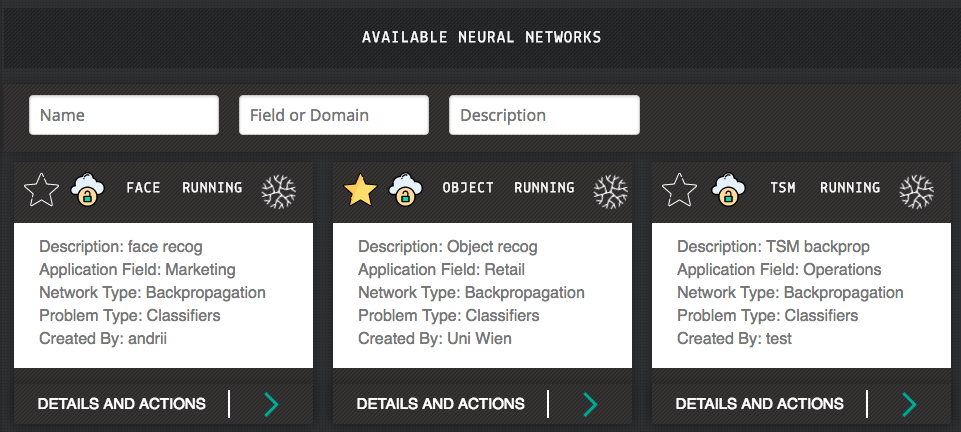
\includegraphics[width=\linewidth]{repo.png}
  \caption{N2Sky neural network repository}
  \label{fig:repo}
  %\vspace*{-30pt}
\end{figure}

Before adding the advised neural networks proposed by the semantic search, the user can inspect the neural network first. The neural network owner can public some training data in order to demonstrate how his neural network behaves. The arbitrary user can also observe the popularity of the neural network, namely how many users performed training against the neural network and if any significant training and evaluation results were published.  

As soon as the user decides that he will add the particular neural network to his project, he can click on copy indicator, which has a star icon form. If the star indicator is grey, users can copy it to their project and perform training and testing on the copied networks. 

Directly after copying the neural network to their own projects, it will be available to the arbitrary user. If the neural network owner modifies the neural network which was added to the project of the arbitrary user, the performed training can be repeated. In case that the neural network owner makes the network private, this network will be hidden from arbitrary user projects. The arbitrary user will always be notified about any occurred changes. 
\item \textbf{Perform the neural network training.} After adding the neural network into its own project, the user can perform training operations. The arbitrary user does not have to know the technical jargon in order to do it. When the user will be on the training screen, the input parameters will be pre-filled with default values as well as default training data nearby attached. With this approach, a user does not need deep knowledge in the neural network field. The N2Sky platform guides the user in order to teach him how the training process works. 
\item \textbf{Add trained model into the project.} The model repository is available to the arbitrary user. Also against trained models can be performed the same way a semantic search as previously done in the neural network repository.The user can preview the trained models and observe the previous testing results. If the model corresponds the users needs, he can add the model to his own project.
\item \textbf{Evaluate the trained models.} The user can perform testing against models trained by himself, as well as copied ones from model repositories. The default testing data will be proposed in order to teach the user how the evaluation process works. The user can modify testing data on demand.
\end{enumerate}

\begin{figure}
  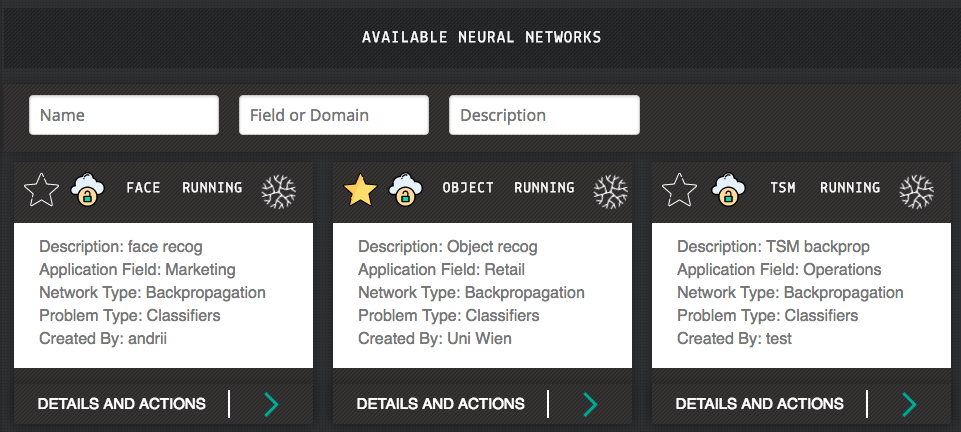
\includegraphics[width=\linewidth]{repo.png}
  \caption{N2Sky neural network repository}
  \label{fig:repo}
  %\vspace*{-30pt}
\end{figure}

 
\subsection{Use Case 2: The Neural Network Engineer}
 % \vspace*{-20pt}

To create a neural network from the paradigm, engineer users have to choose a paradigm and add it to their project. Following steps have to be completed: 
\begin{enumerate}
\item \textbf{Fill out the Neural Network Description form.} Among the available paradigms, the user needs to select one. Every neural network paradigm is defined by the ViNNSL schema. The mandatory fields are name, description, propagation type, learning type, application field and problem type. All this information will be used for semantic searching by other users.
\item \textbf{Define the network structure.} After submitting the Neural Network Description form, the user will be redirected to neural network structure view as shown in figure~\ref{fig:structure}. The structure definition can be customized. It is obligatory to specify the input, hidden and output layers with at least one node in each layer. The number of hidden layers as well as the number of nodes in each layer is unlimited. After defining the network structure, the engineer user has to set connections between nodes. The user can execute full connections as well as add shortcut connections to any node. The users do not need to have any concerns about the correctness of the neural network structure. The application will take care of any errors and mistakes, which users can make.
\begin{figure}[H]
  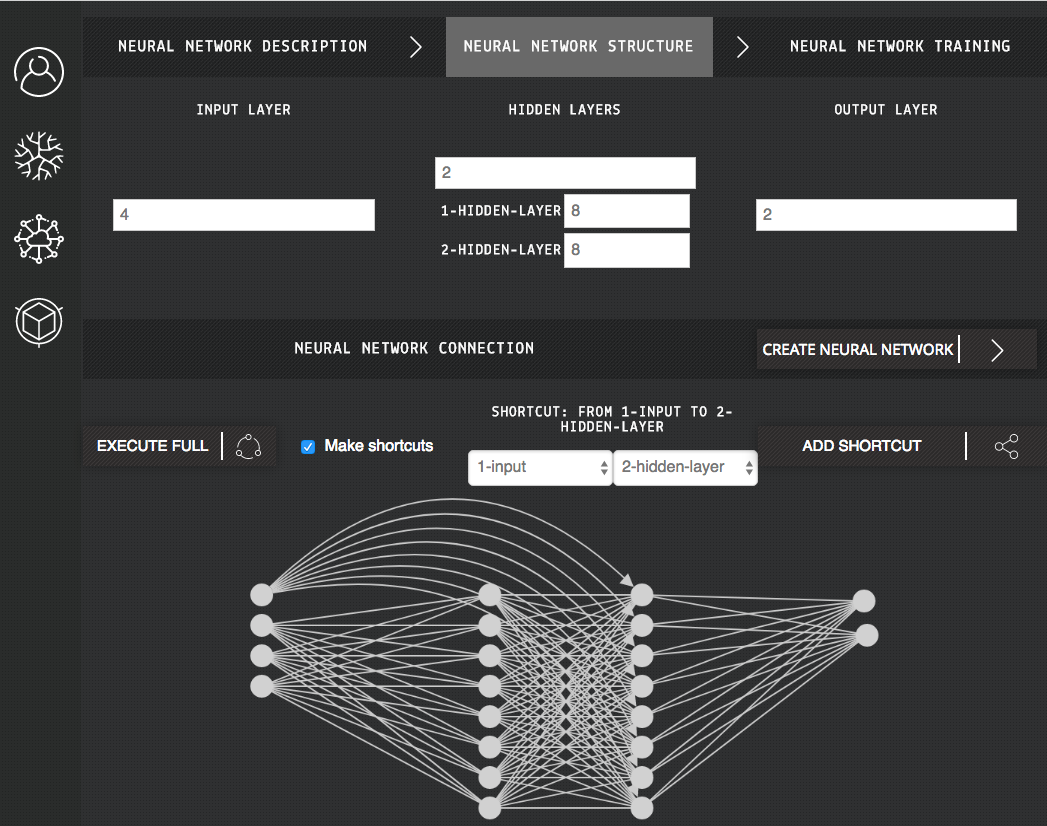
\includegraphics[width=\linewidth]{structure.png}
  \caption{Neural network structure definition}
  \label{fig:structure}
\end{figure}
\item \textbf{Train the newly created neural network and evaluate its model.} After creating a neural network, the users will be redirected to the training view which is shown in figure~\ref{fig:training}. From here, they can run the neural network instance on N2Sky and publish it to make this neural network available for the rest of the users. In case users want to study the neural network in detail, they can also download it in ViNNSL format. Most importantly, users can perform training. Since the neural network was created from the paradigm, default parameters for training are set by default, which guides users through further steps.

\begin{figure}[H]
  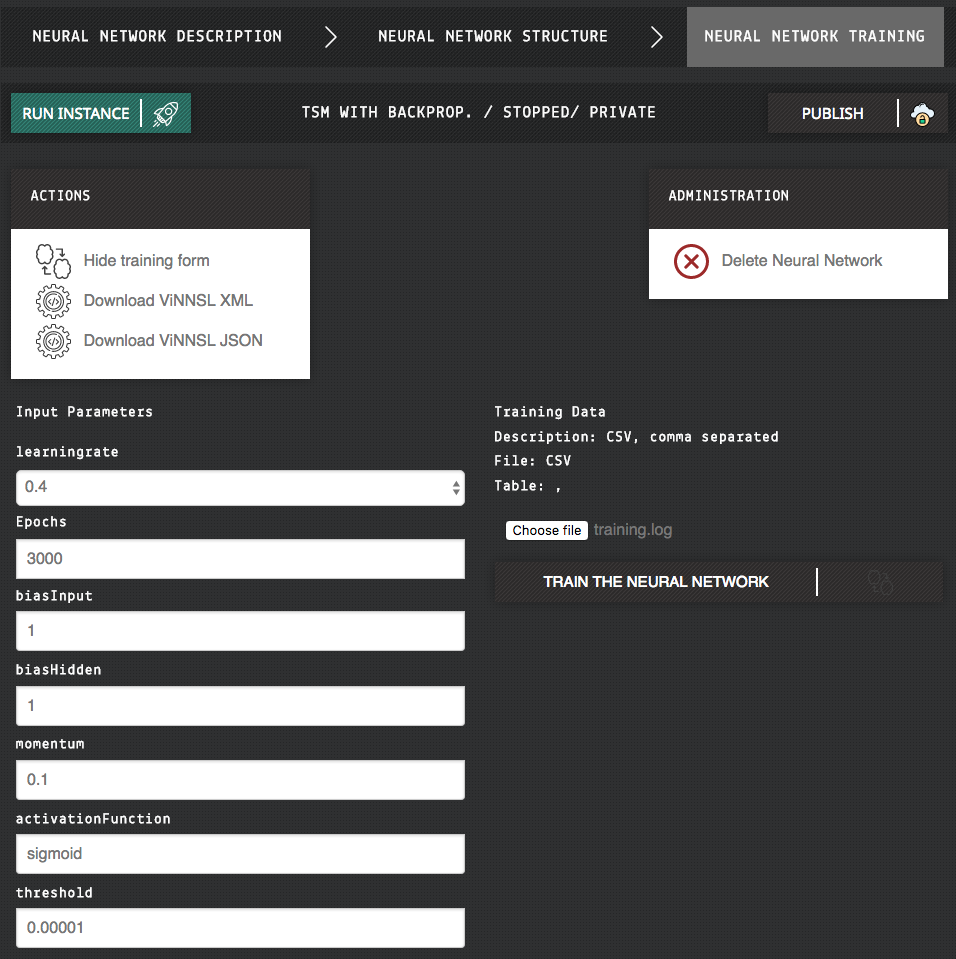
\includegraphics[width=\linewidth]{training.png}
  \caption{Neural network training view}
  \label{fig:training}
\end{figure}




%The training form in figure~\ref{fig:training} shows input parameters, which are needed to perform training. Input parameters as well as requirements for training files are defined in ViNNSL schema.
%Neural network training could take a while, but users will not be blocked. Every evaluation step can be observed in realtime. After training is completed, users can perform testing, see figure~\ref{fig:eval}. The visual representation of evaluation will be shown.  The learning curve is constantly updated during neural network training. The x-Axis shows epochs and the y-Axis shows costs.

After training is completed, users can perform testing, see figure~\ref{fig:eval}. The visual representation of evaluation will be shown. The learning curve is constantly updated during neural network training. The x-Axis shows epochs, and the y-Axis shows costs.

\begin{figure}[H]
  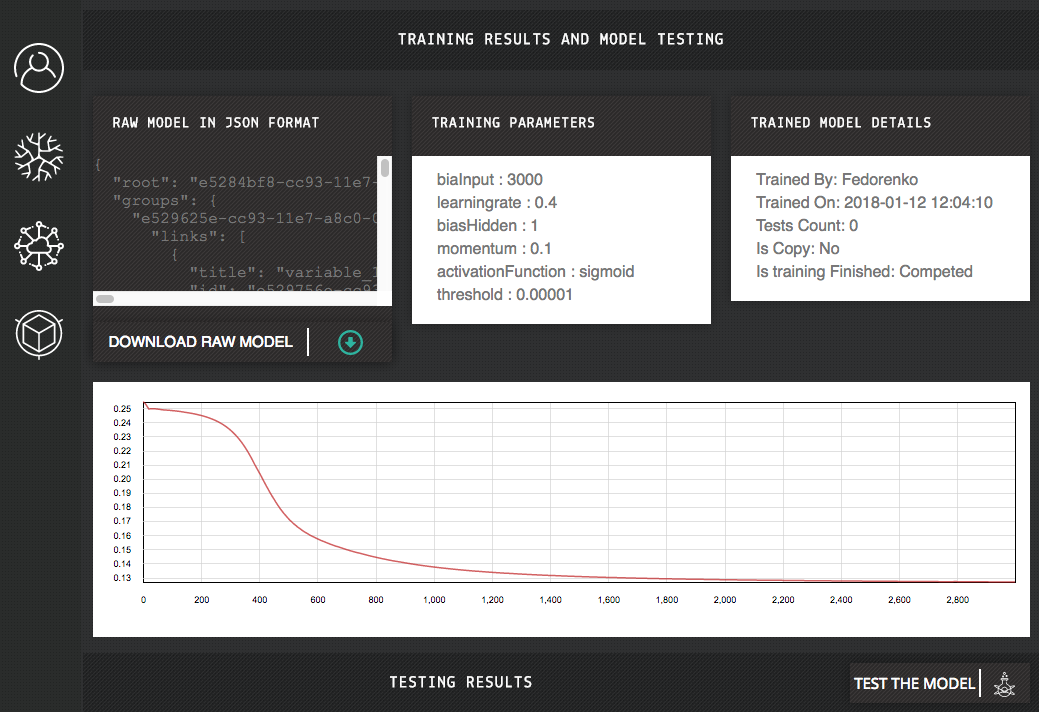
\includegraphics[width=\linewidth]{eval.png}
  \caption{Neural network evaluation process}
  \label{fig:eval}
\end{figure}

\item \textbf{Publish and share the results .} Finally, it is possible to publish and share the trained model so that other users can use it with their own data.

\end{enumerate}



\subsection{Use Case 3: The Neural Network Contributor}

Neural network contributors are expert users. They can download the ViNNSL schema template from N2Sky platform, fill it up and customize their envisioned neural network as shown in figure~\ref{fig:own}. After creating a project, users can just upload their ViNNSL formatted paradigm and deploy it.

\begin{figure}[H]
  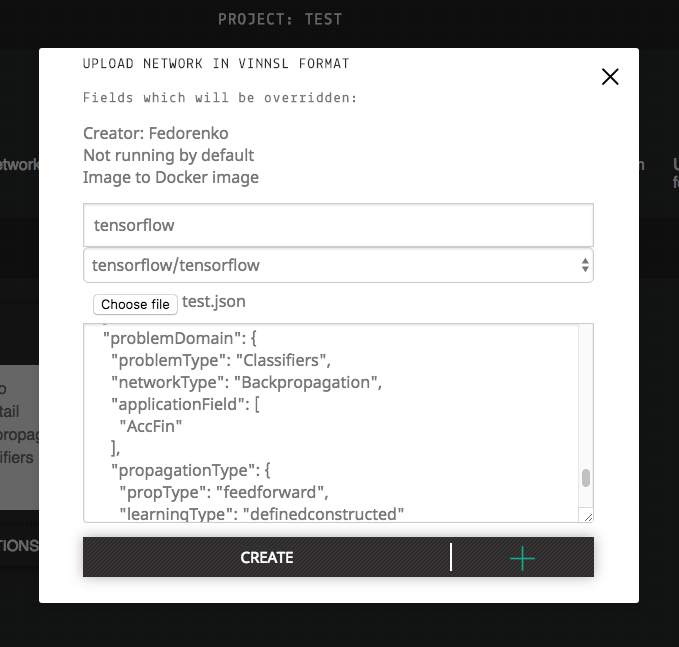
\includegraphics[width=\linewidth]{own_nn.png}
  \caption{Deploying own neural network on N2Sky}
  \label{fig:own}
\end{figure}


Following steps has to be completed in order to publish own neural network paradigm in the N2Sky platform:  
\begin{enumerate}
\item \textbf{Contribute own neural network paradigm.} Since the contributor user is an expert, he will work with a specialised user interface which incorporates technical jargon. Predefined requirements for publishing a users paradigm are the neural network image and the description of this network in ViNNSL format. 

The neural network image has to be a Docker image, which is publicly available in DockerHub repository. N2Sky uses provided Docker images for deploying it into its own cloud. Every image requires the following endpoints:
\begin{itemize}
\item "/train" - endpoint for training a neural network, which provides callback function in order to get the progress results of the training.
\item "/test" - endpoint for evaluation the network, which accepts trained neural network model with requested testing data and responses with evaluating results
\end{itemize}

The description has to be either in ViNNSL XML or ViNNSL JSON format and contain the following predefined components: 
\begin{itemize}
\item General metadata about neural network paradigm.
\item The default structure of neural network and its connections
\item Possible input parameters with default values
\item Type and format of accepted training data
\end{itemize}
ViNNSL template schema allows users to specify which parameters can be edited as well as possible values of particular parameters. The contributor user is free to decide how other people could use his paradigm.

As soon as all pre-requirements are fulfilled, the neural network is available and visible only in the private dashboard of contributor user. 

\item \textbf{Deploy and publish own neural network paradigm.} N2Sky platform gives to contributor users more flexibility. There are two ways how the instance can be run with his own neural network paradigm:
\begin{itemize}
\item Deploy in the N2Sky cloud. For every image with the neural network paradigm, the independent instance in N2Sky cloud will be created. The user provides the publicly available Docker image which will be pulled and deployed in the cloud. 

Since the contributor user wants to know how his neural network will behave during training and evaluation, special monitoring information will be provided. The monitoring charts are available on N2Sky portal as well as via API service. After gathering the monitoring data, the user can adjust the virtual machine environment configuration. Considering that the instance of our neural network is located in the cloud, any adjustment in configuration will be automatically applied without restarting of the instance. 
\item Deploy in an external cloud. If the contributor user decides to keep his own neural network paradigm private, he can publish it on any third party cloud like Amazon Web Services (AWS) or Google Cloud Platform. The user has to provide correct endpoints for training the neural network and testing the trained model. After N2Sky platform validates the reachability of the neural network instance, the contributor user can operate the instance directly from the user interface. 

All functionality, except the instance monitoring, is available. It is also possible to adjust environment configuration because N2Sky can not operate instances in the external cloud. The neural network training and evaluation on trained models can take longer because of the latency between the N2Sky platform and the external cloud. 
\end{itemize}

\item \textbf{Analyse the training and evaluating results of the other users.} 
One of the main purposes of a contributor user is to study the correctness and the behaviour of the provided neural network paradigm. In order to gather this information, the neural network paradigm has to be published on N2Sky platform. As soon as the paradigm becomes available, other users like consumer and neural network engineer ones can start working on it. 

The contributor user is the owner of the neural network instance. Besides monitoring data of the instance environment, the user can observe following information:
\begin{itemize}
\item Observe the training models of the other users against his neural network. The instance owner can audit the training processes of other users, asset some deviations and examine the behaviour of the neural network. 

After gathering the training data of other users, the contributor user can modify his neural network on demand. In this case, the new instance of the neural network will be created and all users who participated in the training of previous versions of this neural network will be notified. The instance owner can retrain his modified neural network with previous users train data. The contributor can perform modification of the neural network and retrain operations multiple times until the training results are satisfying.
\item Observe the evaluation process of the trained models from other users. The contributor user can study the testing results of other users trained models, which were trained against his neural network. The user can distinguish the trained models that offer him the best results. 
\end{itemize}

\end{enumerate}

\section{Summary and Future Research}
\label{sec:summary}

We presented the novel virtual community platform N2Sky, which allows to share and exchange neural network knowledge and computing resources on a worldwide basis by a transparent user-friendly environment. To cope with the ongoing technology shift N2Sky is fostering cloud container technology, which aims for increased extensibility, portability, dynamic orchestration and performance .

In the future, we will extend the focus of N2Sky from the neural network domain to arbitrary machine learning. Hereby a new specification of ViNNSL is under development which aims for compatibility with PMML (Predictive Model Markup Language)~\cite{pmml}. %A further new development of N2Sky is N2Query, which allows the semantic discovery of N2Sky services through a human centered querying mechanism using ontology alignment mechanisms.

%\input{bibl.bbl}

\bibliographystyle{plain}
\bibliography{wcci18}

\end{document}
